\section{Appendix A}\label{appendix-a}\thispagestyle{SectionFirstPage} % Hide headers on the first page of the section
\setcounter{figure}{0}
\setcounter{table}{0}
%
% Logbook
%
\begin{table}[!htbp]
  \footnotesize
  \centering
  \caption{Data collection logbook.}\label{logbook}
  \begin{tabular}{ l l }
  \hline
  Timestamp & Description\\
  \hline
  16/5/2019 14:50:00 & Collection starts\\
  16/5/2019 19:06:00 & Collection starts\\
  17/5/2019 0:39:54 & Collection stops: update current keyword list\\
  17/5/2019 0:46:33 & Collection starts\\
  17/5/2019 15:56:52 & Collection starts\\
  17/5/2019 16:10:52 & Collection starts\\
  18/5/2019 0:00:07 & No. of tweets collected: 865,855 (5.24GB)\\
  19/5/2019 0:40:00 & Secondary collection stops: add tracked topics\\
  19/5/2019 0:42:00 & Secondary collection resumes\\
  19/5/2019 16:50:26 & No. of tweets collected: 2,062,320 (12.73GB)\\
  19/5/2019 22:10:48 & Add \texttt{brexit} as tracked topic\\
  20/5/2019 1:13:40 & Drop \texttt{euthanasia} from hot topics chart; add \texttt{EP2019}\\
  21/5/2019 11:35:52 & Primary collection stops: update KDNP's handle\\
  21/5/2019 11:37:02 & Primary collection resumes\\
  22/5/2019 23:30:13 & eu2019 collection stops\\
  22/5/2019 23:39:41 & eu2019v2 starts\\
  27/5/2019 00:10:27 & eu2019v2 collection stops\\
  27/5/2019 0:21:49 & Insert to eu2019v3 starts\\
  02/6/2019 0:00:00 & All collections terminate\\
  \hline
  \textit{Note: Timezone is CET.}
  \end{tabular}
\end{table}

%
% Topic
%
\begin{table}[!htbp]
  \small
  \centering
  \caption{Topic file for \texttt{refugees}.}
  \label{topic-file}
  \resizebox{0.8\width}{!}{\begin{tabular}{@{\extracolsep{40pt}}ccc}
  \hline
  & Keywords &\\
  \hline
  refugees & \textcyr{избеглице} & menekültek\\
  flóttamenn & utečenci & beguncev\\
  bēgļi & flyktingar & ffoaduriaid\\
  pabėgėliams & immigrati & \textcyr{бежанци}\\
  flyktninger & uprchlíků & flygtninge\\
  uchodźcy & vluchtelingen & põgenikele\\
  refugiados & pakolaisten & immigrés\\
  refugiați & Flüchtlinge & \begin{otherlanguage*}{greek}
  πρόσφυγες
  \end{otherlanguage*}\\
  \hline \\[-1.8ex]
  \end{tabular}}
\end{table}

%
% Nodes table
%
\begin{table}[H]
  \caption{Nodes table for topic: \texttt{refugees}.}\label{nodestable}
  \small
  \begin{center}
  \begin{tabular}{ l l l }
  \hline
  Id & Label\\
  \hline
  1091795183560210000 & AMIRDA1975\\
  1103761100733110000 & maryamnorouzi11\\
  1092802809513290000 & Parisamohajer1\\
  1095035742177380000 & Zgh75204326\\
  707483831331397000 & MarjanG1234\\
  ... & \\
  1095096157401800000 & ODREC\_ONG\\
  140792228 & bentebecker\\
  293418869 & economicsfest\\
  872025895657144000 & LordProvostGCC\\
  161983599 & UNHCRGreece\\
  \hline
  \end{tabular}
  \end{center}
\end{table}

%
% Edges table
%
\begin{table}[H]
  \small
  \caption{Edges table for topic: \texttt{refugees}.}\label{edgestable}
  \begin{center}
  \begin{tabular}{ l l l }
  \hline
  Source & Target & Weight\\
  \hline
  1092802809513290000	& 1091795183560210000	& 4\\
  1092802809513290000	& 1087275641727250000	& 19\\
  1095035742177380000	& 1103761100733110000	& 4\\
  1103761100733110000	& 1103761100733110000	& 3\\
  707483831331397000	& 1103761100733110000	& 2\\
  ... & &\\
  1046126245426140000 & 18393773 & 1\\
  707483831331397000 & 3060125596 & 5\\
  307012746 & 1116005242737500000 & 2\\
  307012746 & 43115163 & 1\\
  307012746 & 3060125596 & 1\\
  \hline
  \end{tabular}
  \end{center}
\end{table}

%
% Metrics table
%
\newpage
\thispagestyle{SectionFirstPage}
\renewcommand{\arraystretch}{3}
\begin{sidewaystable}[!htbp]
  \centering
  \caption{Nodes table with network measures for topic: \texttt{refugees}.}\label{metricstable}
  % Set table width
  \resizebox{0.6\width}{!}{\begin{tabular}{ l l c c c c c c c c c c c c c}
  \hline
  Id & Label & Indegree & Outdegree & Degree & \makecell{Weighted\\indegree} & \makecell{Weighted\\outdegree} & \makecell{Weighted\\degree} & Eccentricity & \makecell{Closness\\centrality} & \makecell{Harmonic\\closness\\centrality} & \makecell{Betweeness\\centrality} & Modularity & Clustering & Eigencentrality\\
  \hline
  1091795183560210000 & AMIRDA1975 & 23 & 43 & 66 & 106 & 92 & 198 & 6 & .404408 & .451794 & 69269621413 & 2 & .181186 & .348815\\
  1103761100733110000 & maryamnorouzi11 & 15 & 9 & 24 & 47 & 18 & 65 & 6 & .381894 & .414124 & 756181729 & 2 & .45 & .231786\\
  1092802809513290000 & Parisamohajer1 & 87 & 118 & 205 & 289 & 360 & 649 & 6 & .464263 & .533878 & 45579722672 & 2 & .065114 & .555289\\
  1095035742177380000 & Zgh75204326 & 54 & 181 & 235 & 242 & 766 & 1008 & 6 & .496281 & .585195 & 53321060569 & 2 & .054794 & .548923\\
  707483831331397000 & MarjanG1234 & 213 & 209 & 422 & 724 & 894 & 1618 & 6 & .509015 & .605472 & 213888327949 & 2 & .027361 & .750295\\
  ... & \\
  1095096157401800000 & ODREC\_ONG & 1 & 0 & 1 & 1 & 0 & 1 & 0 & 0 & 0 & 0 & 2 & 0 & .000562\\
  140792228 & bentebecker & 1 & 0 & 1 & 1 & 0 & 1 & 0 & 0 & 0 & 0 & 2 & 0 & .000562\\
  293418869 & economicsfest & 1 & 0 & 1 & 1 & 0 & 1 & 0 & 0 & 0 & 0 & 2 & 0 & .001731\\
  872025895657144000 & LordProvostGCC & 1 & 0 & 1 & 1 & 0 & 1 & 0 & 0 & 0 & 0 & 2 & 0 & .000562\\
  161983599 & UNHCRGreece & 1 & 0 & 1 & 1 & 0 & 1 & 0 & 0 & 0 & 0 & 2 & 0 & .000562\\
  \hline
  \end{tabular}}
\end{sidewaystable}
\renewcommand{\arraystretch}{1.5}

%
% Brexit summary
%
\begin{table}[!htbp]
  \centering
  \small
  \caption{Summary statistics for topic: \texttt{brexit}.}
  \label{brexitsummary}
  \resizebox{0.8\width}{!}{\begin{tabular}{@{\extracolsep{5pt}}lccccccc}
  \hline
  Statistic & \multicolumn{1}{c}{N} & \multicolumn{1}{c}{Mean} & \multicolumn{1}{c}{St. Dev.} & \multicolumn{1}{c}{Min} & \multicolumn{1}{c}{Pctl(25)} & \multicolumn{1}{c}{Pctl(75)} & \multicolumn{1}{c}{Max} \\
  \hline \\[-1.8ex]
  indegree & 4,843 & 1.905 & 7.165 & 0 & 0 & 1 & 211 \\
  outdegree & 4,843 & 1.905 & 3.938 & 0 & 0 & 3 & 76 \\
  degree & 4,843 & 3.810 & 7.806 & 1 & 1 & 4 & 211 \\
  weighted\_indegree & 4,843 & 2.711 & 10.798 & 0 & 0 & 2 & 274 \\
  weighted\_outdegree & 4,843 & 2.711 & 6.094 & 0 & 0 & 4 & 121 \\
  weighted\_degree & 4,843 & 5.422 & 12.012 & 1 & 1 & 5 & 274 \\
  eccentricity & 4,843 & .441 & .642 & 0 & 0 & 1 & 4 \\
  closnesscentrality & 4,843 & .353 & .466 & 0 & 0 & 1 & 1 \\
  harmonic\_closness\_centrality & 4,843 & .357 & .469 & 0 & 0 & 1 & 1 \\
  betweenesscentrality & 4,843 & .751 & 16.555 & 0 & 0 & 0 & 790 \\
  clustering & 4,843 & .004 & .031 & 0 & 0 & 0 & 0 \\
  eigencentrality & 4,843 & .009 & .036 & 0 & 0 & .01 & 1 \\
  \hline \\[-1.8ex]
  \multicolumn{8}{l}{\textit{Number of nodes = 4,843; Number of edges = 9,226.}}
\end{tabular}}
\end{table}

%
% Populism summary
%
\begin{table}[!htbp]
  \centering
  \small
  \caption{Summary statistics for topic: \texttt{populism}.}
  \label{populismsummary}
  \resizebox{0.8\width}{!}{\begin{tabular}{@{\extracolsep{5pt}}lccccccc}
  \hline
  Statistic & \multicolumn{1}{c}{N} & \multicolumn{1}{c}{Mean} & \multicolumn{1}{c}{St. Dev.} & \multicolumn{1}{c}{Min} & \multicolumn{1}{c}{Pctl(25)} & \multicolumn{1}{c}{Pctl(75)} & \multicolumn{1}{c}{Max} \\
  \hline \\[-1.8ex]
  indegree & 704 & 1.950 & 4.746 & 0 & 0 & 2 & 53 \\
  outdegree & 704 & 1.950 & 1.987 & 0 & 0 & 3 & 16 \\
  degree & 704 & 3.901 & 4.545 & 1 & 2 & 4 & 53 \\
  weighted\_indegree & 704 & 4.470 & 10.809 & 0 & 0 & 4 & 145 \\
  weighted\_outdegree & 704 & 4.470 & 5.318 & 0 & 0 & 8 & 72 \\
  weighted\_degree & 704 & 8.940 & 11.170 & 1 & 4 & 10 & 145 \\
  eccentricity & 704 & .751 & .829 & 0 & 0 & 1 & 5 \\
  closness\_centrality & 704 & .501 & .467 & 0 & 0 & 1 & 1 \\
  harmonic\_closness\_centrality & 704 & .515 & .474 & 0 & 0 & 1 & 1 \\
  betweeness\_centrality & 704 & .555 & 3.573 & 0 & 0 & 0 & 42 \\
  clustering & 704 & .042 & .101 & 0 & 0 & 0 & 0 \\
  eigencentrality & 704 & .032 & .106 & 0 & 0 & .01 & 1 \\
  \hline \\[-1.8ex]
  \multicolumn{8}{l}{\textit{Number of nodes = 704; Number of edges = 1,373.}}
\end{tabular}}
\end{table}

%
% Refugees summary
%
\begin{table}[!htbp]
  \centering
  \small
  \caption{Summary statistics for topic: \texttt{refugees}.}
  \label{refugeessummary}
  \resizebox{0.8\width}{!}{\begin{tabular}{@{\extracolsep{5pt}}lccccccc}
  \hline
  Statistic & \multicolumn{1}{c}{N} & \multicolumn{1}{c}{Mean} & \multicolumn{1}{c}{St. Dev.} & \multicolumn{1}{c}{Min} & \multicolumn{1}{c}{Pctl(25)} & \multicolumn{1}{c}{Pctl(75)} & \multicolumn{1}{c}{Max} \\
  \hline \\[-1.8ex]
  indegree & 2,952 & 4.725 & 16.975 & 0 & 0 & 2 & 430 \\
  outdegree & 2,952 & 4.725 & 14.191 & 0 & 0 & 4 & 265 \\
  degree & 2,952 & 9.451 & 24.953 & 1 & 3 & 5 & 430 \\
  weighted\_indegree & 2,952 & 9.395 & 49.085 & 0 & 0 & 3 & 1,614 \\
  weighted\_outdegree & 2,952 & 9.395 & 46.012 & 0 & 0 & 5 & 1,120 \\
  weighted\_degree & 2,952 & 18.791 & 81.807 & 1 & 4 & 7 & 1,864 \\
  eccentricity & 2,952 & 2.932 & 3.238 & 0 & 0 & 7 & 10 \\
  closness\_centrality & 2,952 & .358 & .378 & 0.000 & 0.000 & .643 & 1.000 \\
  harmonic\_closness\_centrality & 2,952 & .371 & .382 & 0.000 & 0.000 & .750 & 1.000 \\
  betweeness\_centrality & 2,952 & 665.544 & 6,589.509 & 0.000 & 0.000 & 0.000 & 213,888.300 \\
  clustering & 2,952 & .094 & .177 & 0.000 & 0.000 & .160 & 1.000 \\
  eigencentrality & 2,952 & .026 & .081 & 0.000 & 0.000 & .003 & 1.000 \\
  \hline \\[-1.8ex]
  \multicolumn{8}{l}{\textit{Number of nodes = 2,952; Number of edges = 13,949.}}
\end{tabular}}
\end{table}

%
% Terrorism summary
%
\begin{table}[!htbp]
  \centering
  \small
  \caption{Summary statistics for topic: \texttt{terrorism}.}
  \label{terrorismsummary}
  \resizebox{0.8\width}{!}{\begin{tabular}{@{\extracolsep{5pt}}lccccccc}
  \hline
  Statistic & \multicolumn{1}{c}{N} & \multicolumn{1}{c}{Mean} & \multicolumn{1}{c}{St. Dev.} & \multicolumn{1}{c}{Min} & \multicolumn{1}{c}{Pctl(25)} & \multicolumn{1}{c}{Pctl(75)} & \multicolumn{1}{c}{Max} \\
  \hline \\[-1.8ex]
  indegree & 2,033 & 2.224 & 6.831 & 0 & 0 & 2 & 93 \\
  outdegree & 2,033 & 2.224 & 1.925 & 0 & 0 & 3 & 15 \\
  degree & 2,033 & 4.448 & 6.588 & 1 & 3 & 4 & 97 \\
  weighted\_indegree & 2,033 & 4.029 & 12.562 & 0 & 0 & 4 & 216 \\
  weighted\_outdegree & 2,033 & 4.029 & 3.850 & 0 & 0 & 8 & 35 \\
  weighted\_degree & 2,033 & 8.058 & 12.334 & 1 & 4 & 8 & 216 \\
  eccentricity & 2,033 & 1.038 & 1.040 & 0 & 0 & 2 & 6 \\
  closness\_centrality & 2,033 & .541 & .434 & 0 & 0 & 1 & 1 \\
  harmonic\_closness\_centrality & 2,033 & .566 & .440 & 0 & 0 & 1 & 1 \\
  betweeness\_centrality & 2,033 & 1.973 & 20.934 & 0 & 0 & 0 & 470 \\
  clustering & 2,033 & .034 & .090 & 0 & 0 & 0 & 0 \\
  eigencentrality & 2,033 & .013 & .047 & 0 & 0 & .01 & 1 \\
  \hline \\[-1.8ex]
  \multicolumn{8}{l}{\textit{Number of nodes = 2,033; Number of edges = 4,521.}}
\end{tabular}}
\end{table}

%
% Unemployment summary
%
\begin{table}[!htbp]
  \small
  \centering
  \caption{Summary statistics for topic: \texttt{unemployment}.}
  \label{unemploymentsummary}
  \resizebox{0.8\width}{!}{\begin{tabular}{@{\extracolsep{5pt}}lccccccc}
  \hline
  Statistic & \multicolumn{1}{c}{N} & \multicolumn{1}{c}{Mean} & \multicolumn{1}{c}{St. Dev.} & \multicolumn{1}{c}{Min} & \multicolumn{1}{c}{Pctl(25)} & \multicolumn{1}{c}{Pctl(75)} & \multicolumn{1}{c}{Max} \\
  \hline \\[-1.8ex]
  indegree & 1,406 & 2.370 & 10.014 & 0 & 0 & 1 & 166 \\
  outdegree & 1,406 & 2.370 & 2.124 & 0 & 0 & 3 & 19 \\
  degree & 1,406 & 4.740 & 9.865 & 1 & 3 & 3 & 169 \\
  weighted\_indegree & 1,406 & 3.322 & 14.036 & 0 & 0 & 2 & 257 \\
  weighted\_outdegree & 1,406 & 3.322 & 3.339 & 0 & 0 & 4 & 50 \\
  weighted\_degree & 1,406 & 6.644 & 13.884 & 1 & 4 & 5 & 257 \\
  eccentricity & 1,406 & 1.165 & 1.075 & 0 & 0 & 2 & 4 \\
  closness\_centrality & 1,406 & .571 & .421 & 0 & 0 & 1 & 1 \\
  harmonic\_closness\_centrality & 1,406 & .599 & .426 & 0 & 0 & 1 & 1 \\
  betweeness\_centrality & 1,406 & 2.142 & 24.824 & 0 & 0 & 0 & 692 \\
  clustering & 1,406 & .027 & .079 & 0 & 0 & 0 & 0 \\
  eigencentrality & 1,406 & .013 & .055 & 0 & 0 & .004 & 1 \\
  \hline \\[-1.8ex]
  \multicolumn{8}{l}{\textit{Number of nodes = 1,406; Number of edges = 3,332.}}
\end{tabular}}
\end{table}

\clearpage
\begin{figure}
    \centering
    \caption{Bivariate correlation matrix for topic: \texttt{populism}.}\label{corr-matrix-populism}
    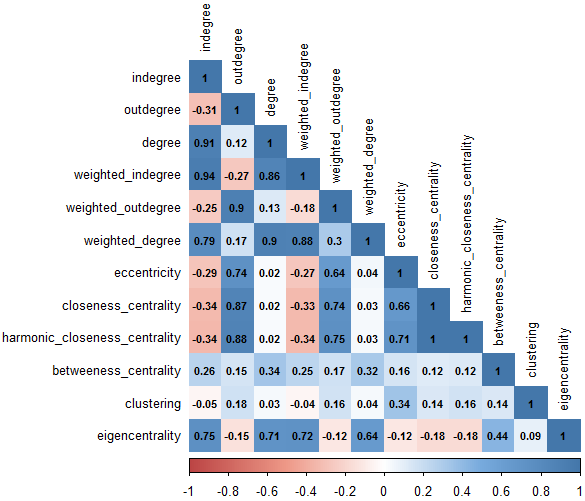
\includegraphics[width=.8\textwidth]{corr-matrix-populism}
\end{figure}
\begin{figure}
  \centering
  \caption{Bivariate correlation matrix for topic: \texttt{refugees}.}\label{corr-matrix-refugees}
  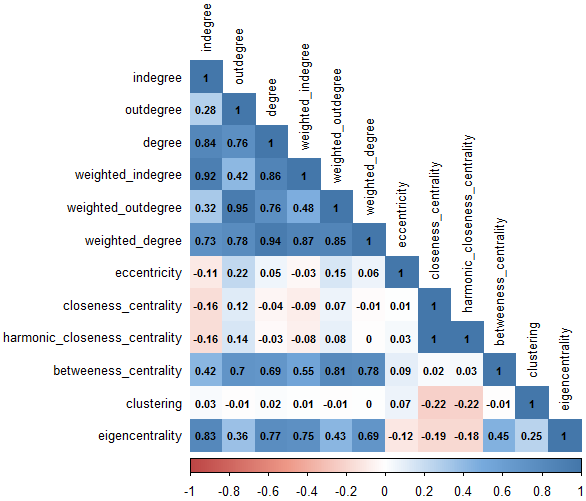
\includegraphics[width=.8\textwidth]{corr-matrix-refugees}
\end{figure}

\clearpage
\begin{figure}
  \centering
  \caption{Bivariate correlation matrix for topic: \texttt{terrorism}.}\label{corr-matrix-terrorism}
  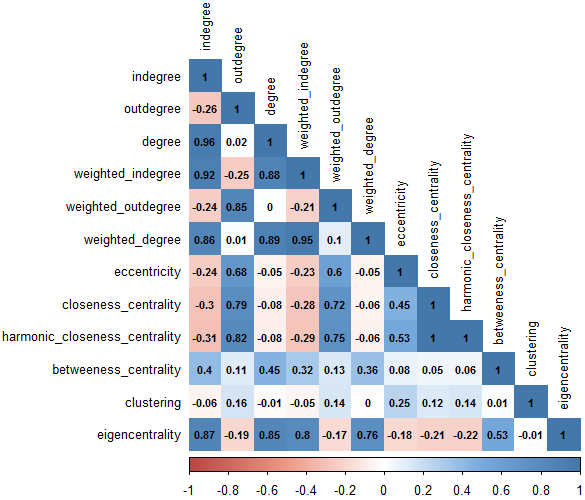
\includegraphics[width=.8\textwidth]{corr-matrix-terrorism}
\end{figure}
\begin{figure}
  \centering
  \caption{Bivariate correlation matrix for topic: \texttt{unemployment}.}\label{corr-matrix-unemployment}
  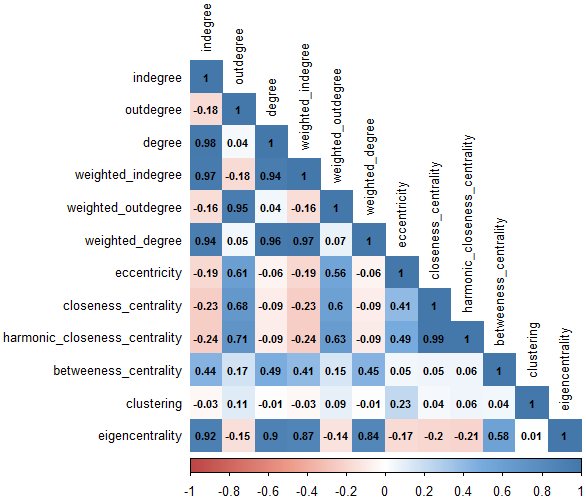
\includegraphics[width=.8\textwidth]{corr-matrix-unemployment}
\end{figure}

\clearpage
\thispagestyle{SectionFirstPage}
\begin{sidewaysfigure}[ht]
  \caption{Coefficients and SE per topic of Model A (Complete OLS).\label{model-a-coeff}}
  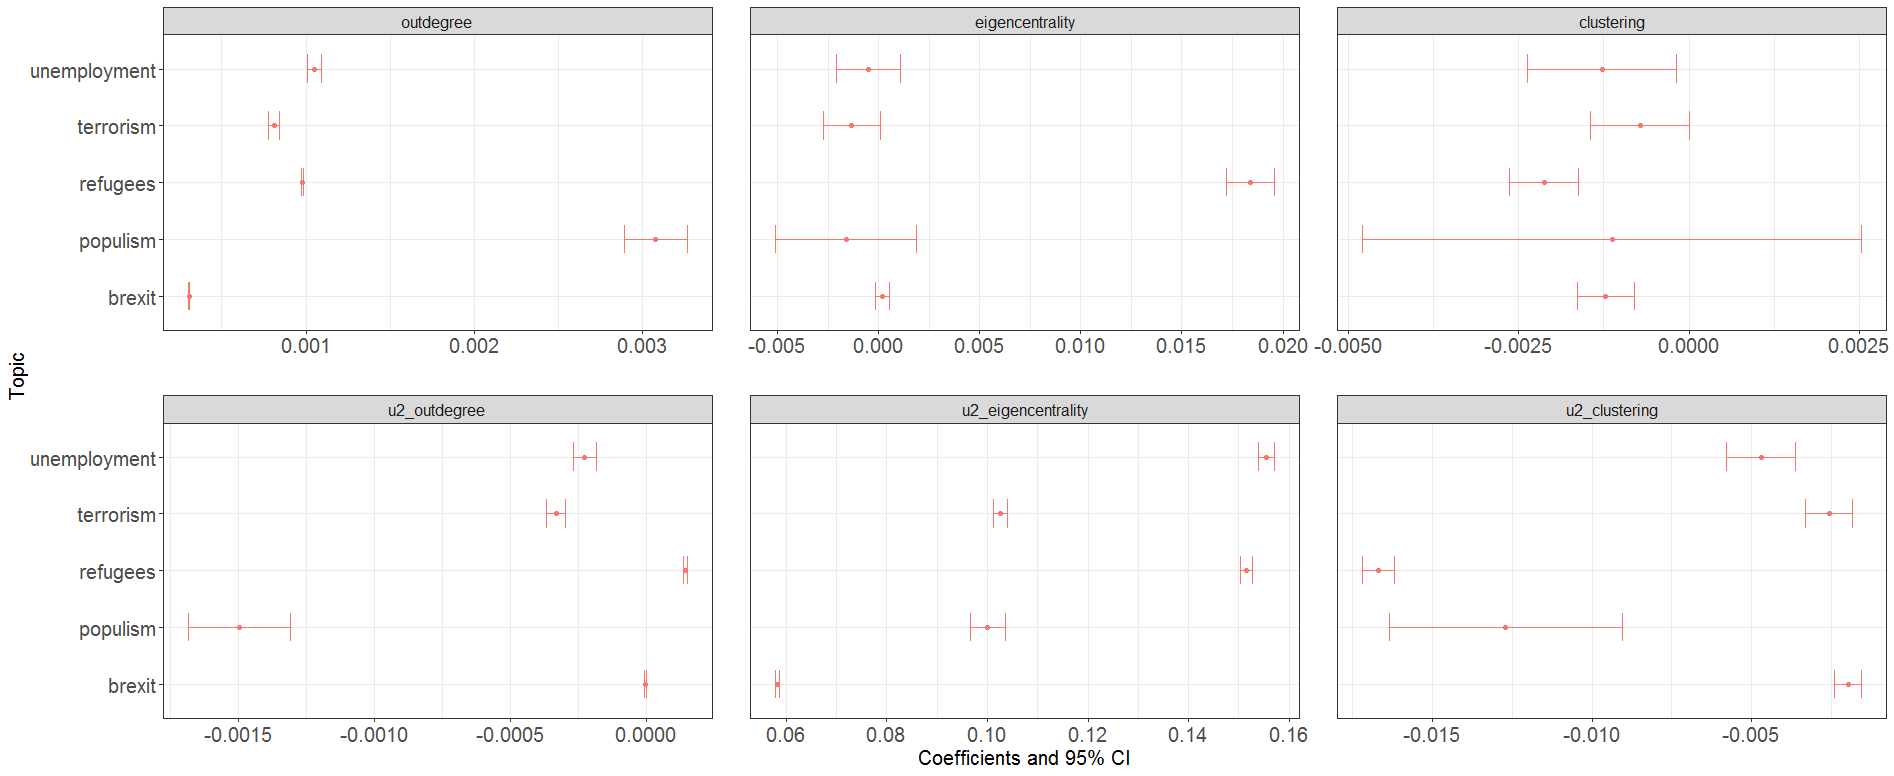
\includegraphics[width=\textwidth]{model_A_coeff}
\end{sidewaysfigure}

\clearpage
\thispagestyle{SectionFirstPage}
\begin{sidewaysfigure}[ht]
  \caption{Coefficients and SE per topic of Model B (Logistic).\label{model-b-coeff}}
  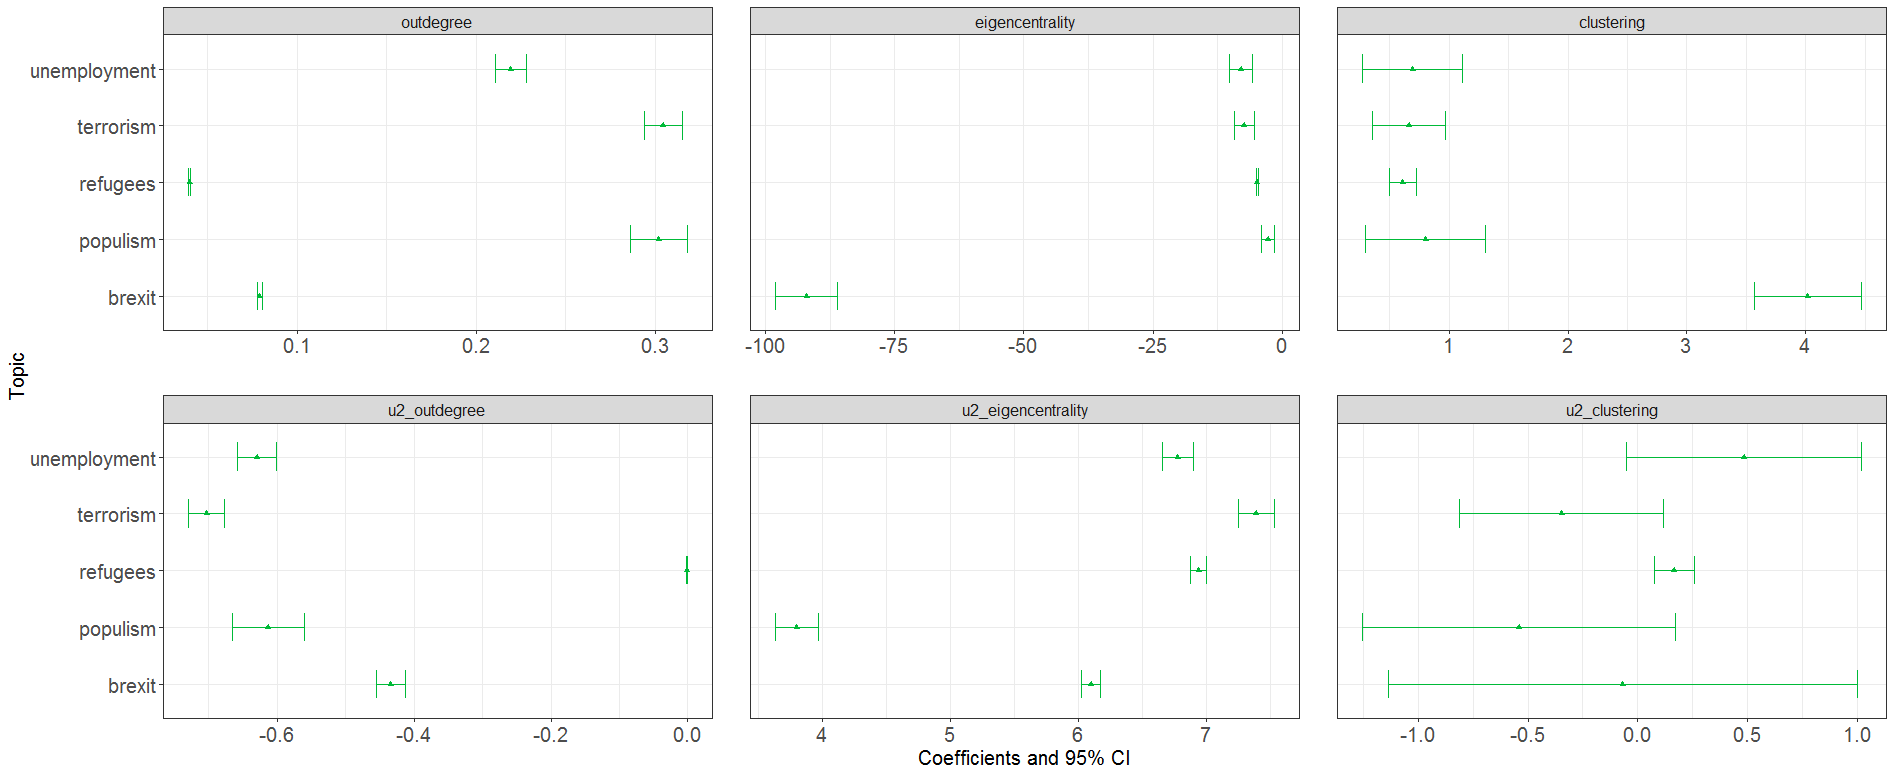
\includegraphics[width=\textwidth]{model_B_coeff}
\end{sidewaysfigure}

\clearpage
\thispagestyle{SectionFirstPage}
\begin{sidewaysfigure}[ht]
  \caption{Coefficients and SE per topic of Model C (Conditional OLS).\label{model-c-coeff}}
  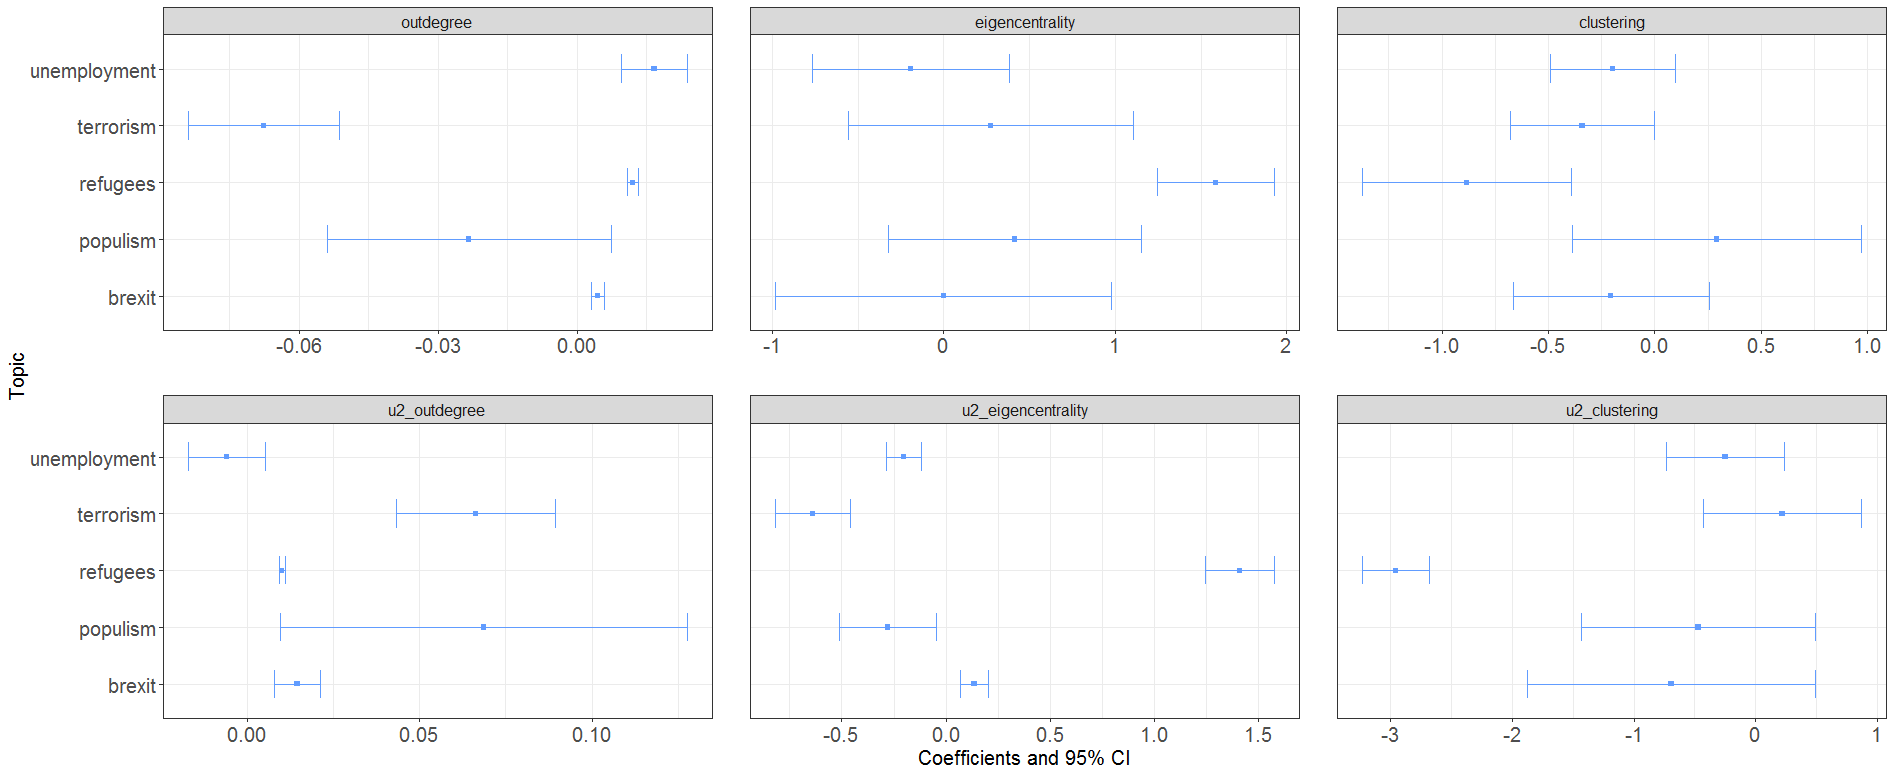
\includegraphics[width=\textwidth]{model_C_coeff}
\end{sidewaysfigure}
